%%&program=xelatex
%&encoding=UTF-8 Unicode
% SVN keywords
% $Author$
% $Date$
% $Revision$
% $URL$
\documentclass[a4paper,12pt]{article}  % Comments after  % are ignored
%\usepackage{hyperref}                 % For creating hyperlinks in cross references
%
\usepackage{ifxetex}% for XELATEX, or PDFlatex
\usepackage{ifplatform} 
%
\ifxetex
	\usepackage{polyglossia} \setmainlanguage{portuges}
	\usepackage{fontspec}
	\ifwindows
		\setmainfont[Ligatures=TeX]{Garamond}
		\setsansfont[Ligatures=TeX]{Gill Sans MT}
		\setmonofont[Scale=MatchLowercase]{Courier}
	\fi
	\iflinux
		\setmainfont[Ligatures=TeX]{Linux Libertine O}
		\setsansfont[Ligatures=TeX,Scale=MatchLowercase]{Linux Biolinum}
		\setmonofont[Scale=MatchLowercase]{Courier}
	\fi
	\ifmacosx
	% add settings
	% Use xelatex -no-shell ...
	\fi
	\usepackage{xcolor,graphicx} 
\else
	\usepackage[portuguese]{babel}
	%\usepackage[latin1]{inputenc}
	\usepackage[utf8]{inputenc}
	\usepackage[T1]{fontenc}
	\usepackage{graphics}                 % Packages to allow inclusion of graphics
	\usepackage{color}                    % For creating coloured text and background
\fi

\usepackage{enumitem}
\setlist{nolistsep}

\usepackage{amsmath,amssymb,amsfonts} % Typical maths resource packages
\usepackage[retainorgcmds]{IEEEtrantools}
\usepackage{caption}


\oddsidemargin 0cm
\evensidemargin 0cm

\pagestyle{myheadings}         % Option to put page headers
                               % Needed \documentclass[a4paper,twoside]{article}
\markboth{{\small \it  Laboratório de Física Experimental Básica}}
{{\small\it MEFT - 1º Sem. 2013/2014} }

\addtolength{\hoffset}{-0.5cm}
\addtolength{\textwidth}{2.5cm}
\addtolength{\topmargin}{-1.5cm}
\addtolength{\textheight}{3cm}

%\textwidth 15.5cm
%\topmargin -1.5cm
\setlength{\parindent}{0pt}
\setlength{\parskip}{1ex  plus  0.5ex  minus  0.2ex}
%\parindent 0.5cm
%\textheight 25cm
%\parskip 1mm


% Math macros
\newcommand{\ud}{\,\mathrm{d}} 
\newcommand{\HRule}{\rule{\linewidth}{0.5mm}}

\author{Prof. Bernardo B. Carvalho} 

%%%%, Bernardo Brotas Carvalho\\bernardo@ipfn.ist.utl.pt} 
\date{ Outubro 2012} 

\begin{document} 

	
\includegraphics[width=0.2\textwidth]{../logo-ist}%\\[1cm]  %%  Logo_IST_color

	\HRule \\[0.5cm]
	{ \huge \sf  \textsc{Indice de Refração do vidro de um Prisma pelo método  do Desvio Mínimo.}} \\[0.4cm] % \bfseries 
%	{ \huge \sf  \textsc{Construções Geométricas em Lentes Delgadas (aproximação paraxial)} }\\[0.4cm] % \bfseries 
	{ \large \bfseries Poder Dispersivo do Vidro. Poder de Resolução.}\\
%	{ \large \bfseries Procedimento Experimental}\\
	\HRule \\%[0.5cm]

\section{\sf Princípio do método}
Um prisma de um meio transparente, homogéneo e isótropo de índice de refração, $n$, colocado no percurso de um feixe luminoso incidente produz um desvio angular no feixe emergente que depende do ângulo de incidência. Pode provar-se facilmente que esse desvio angular apresenta um ponto de estacionariedade (i.e., derivada nula) que é um mínimo se $n > 1$. 
Essa situação acontece quando as direções dos dois feixes são igualmente inclinadas em relação às faces do prisma, i.e. quando o ângulo de incidência é igual ao ângulo de transmissão 
emergente (ver Apêndice). 
Nesse caso  (Figura \ref{fig:angulo}) o índice de refração, $n$, pode ser calculado simplesmente através da expressão seguinte: 

\begin{equation}
	\label{eq:desviomim}
	n= \frac{\sin \left( \frac{\alpha+ \delta_{min}}{2} \right) } {\sin \left(  \frac{\alpha}{2} \right)}  
\end{equation}

em que $\alpha$ e  $\delta_{min}$ são os ângulos, respetivamente, do prisma e do desvio mínimo referido. Este desvio mínimo depende do comprimento de onda da radiação incidente, $\lambda$, e por consequência $n$ depende de $\lambda$. Define-se \emph{poder dispersivo} dum material como a derivada de $n$ em ordem a $\lambda$. Como esta função não é linear, deve indicar-se o valor do poder dispersivo relativo a um determinado valor de comprimento de onda incidente,  $\lambda_i$,  e escreve-se pois como $\left( \frac{\ud n}{\ud \lambda } \right)_{\lambda_i}$.

O poder separador ou poder de resolução de um instrumento óptico\footnote{Optical Resolution}, $R_\lambda = \frac{\lambda}{\Delta \lambda} $,  é a capacidade que possui de poder permitir que se observem separadamente dois comprimentos de onda muito próximos, afastados de Δλ, na vizinhança de um valor médio λ. Esta grandeza é adimensional e quanto maior for o seu valor, melhor é a resolução do instrumento.

No caso de um prisma obtém-se para $R$ a seguinte expressão (ver Apêndice), se a fonte é linear e se dispõe paralelamente à aresta do prisma:
 \begin{equation}
	\label{eq:resolu}
	R_\lambda = l\,\left(\frac{\ud n}{\ud \lambda} \right)_\lambda 
\end{equation}

em que $l$ é o \emph{maior percurso} do feixe luminoso no interior do prisma.

Uma \emph{rede de difração} (ver apontamentos da Aula Teórica  “Interferência e Difração”) permite também observar separadamente dois comprimentos de onda muito próximos.
Mas para uma rede de difração linear a resolução além de variar com o comprimento de onda depende da \emph{ordem de difração}, $m$
 \begin{equation}
	\label{eq:resoludrifa}
	R_\lambda = m\,N 
\end{equation}
sendo $N$  o número de linhas da rede iluminadas pelo feixe.


\section{\sf A experiência}
\subsection{\sf Equipamento}

\begin{enumerate}
\item Goniómetro de Babinet com prisma,
\item Lâmpada espetral de Mercúrio ou Hélio.
\end{enumerate}

Quando se coloca o prisma na plataforma de modo a poderem observar-se as reflexões nas faces que delimitam o prisma óptico, as direções dos raios refletidos fazem um ângulo $\theta$, que se mede com o goniómetro (Figura \ref{fig:spectrometer}), que é o dobro do ângulo α do prisma. Pode assim determinar-se facilmente o ângulo do prisma e com uma precisão muito melhor do que com um goniómetro de funcionamento mecânico, ou transferidor.

\begin{figure}[tb]  \centering 
	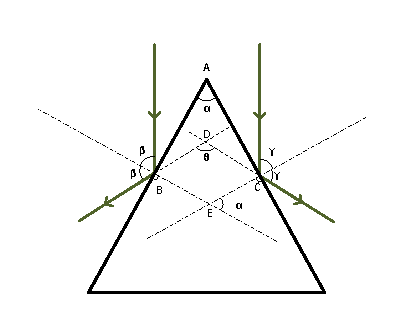
\includegraphics[width=0.6\textwidth]{angulo}
	\caption{Esquema da reflexão do feixe incidente num prisma colocado na plataforma do goniómetro de Babinet. As direções dos dois raios refletidos fazem entre si um ângulo θ que é o dobro do ângulo α do prisma. \label{fig:angulo}} 
\end{figure}

Pode determinar-se o ângulo $\delta_{min}$ medindo a direção do raio incidente (sem prisma) e a direção do raio emergente segundo o ângulo $i_2$ em relação à normal (que corresponda ao desvio mínimo) para cada comprimento de onda (Figura \ref{fig:desvio}). Mas devem fazer-se observações para os raios que emergem das duas faces que definem o ângulo do prisma. Neste caso, e como é facil provar que o ângulo formado pelos dois raios emergentes (para a mesma côr) é o dobro do ângulo de desvio, não é necessário determinar a direção do raio incidente, $i_1$.

O goniómetro é um instrumento que permite medir ângulos. O goniómetro de Babinet tem uma forma central quase cilíndrica (a base) com uma plataforma que roda em torno do eixo (vertical) da base e onde é colocado um prisma (ou uma rede de difração) (Figura \ref{fig:spectrometer}). O goniómetro vem equipado com dois elementos ópticos: um colimador e uma luneta, que estão ambos montados radialmente, o colimador fixo e a luneta podendo rodar em torno do eixo da base (Figura 4). As posições angulares da plataforma (e portanto do prisma) e da luneta podem ser lidas num limbo graduado por intermédio de nónios solidários respetivamente com a plataforma e a luneta. Existem dois parafusos micrométricos, cada um associado a cada um dos nónios que permitem com facilidade fazer leituras das posições angulares, com resolução de $30''$ (meio minuto).

\begin{figure}[tb]  \centering 
	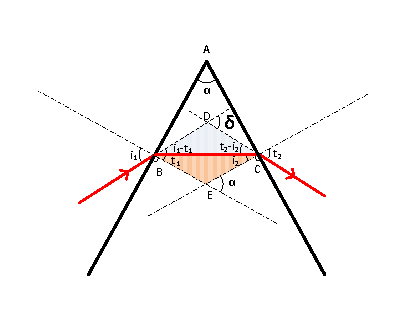
\includegraphics[width=0.6\textwidth]{desvio}
	\caption{Esquema da transmissão do feixe incidente num prisma colocado na plataforma do goniómetro de Babinet. A direção do feixe transmitido desvia-se da direção do feixe incidente do ângulo $\delta$. \label{fig:desvio}} 
\end{figure}

\begin{figure}[tb]  
\centering 
	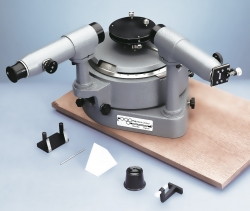
\includegraphics[width=0.45\textwidth]{spectrometer}
	\caption{Fotografia do goniómetro de Babinet (modelo Philipe Harris Advanced Spectrometer 30). \label{fig:spectrometer}} 
\end{figure}

O colimador é constituido por dois tubos cilíndricos concêntricos que se podem deslocar axialmente. Um deles possui uma fenda retilínea de largura variável e que deve ser colocada na vertical. O outro, tem em posição oposta, i.e. mais próximo da região central, uma lente convergente. O objetivo deste conjunto, quando a fenda é iluminada por uma fonte luminosa divergente, é produzir um feixe paralelo na região da plataforma. A fenda vai funcionar como objeto linear se a fenda for relativamente estreita.

\begin{figure}[!htb]  
	\centering 
	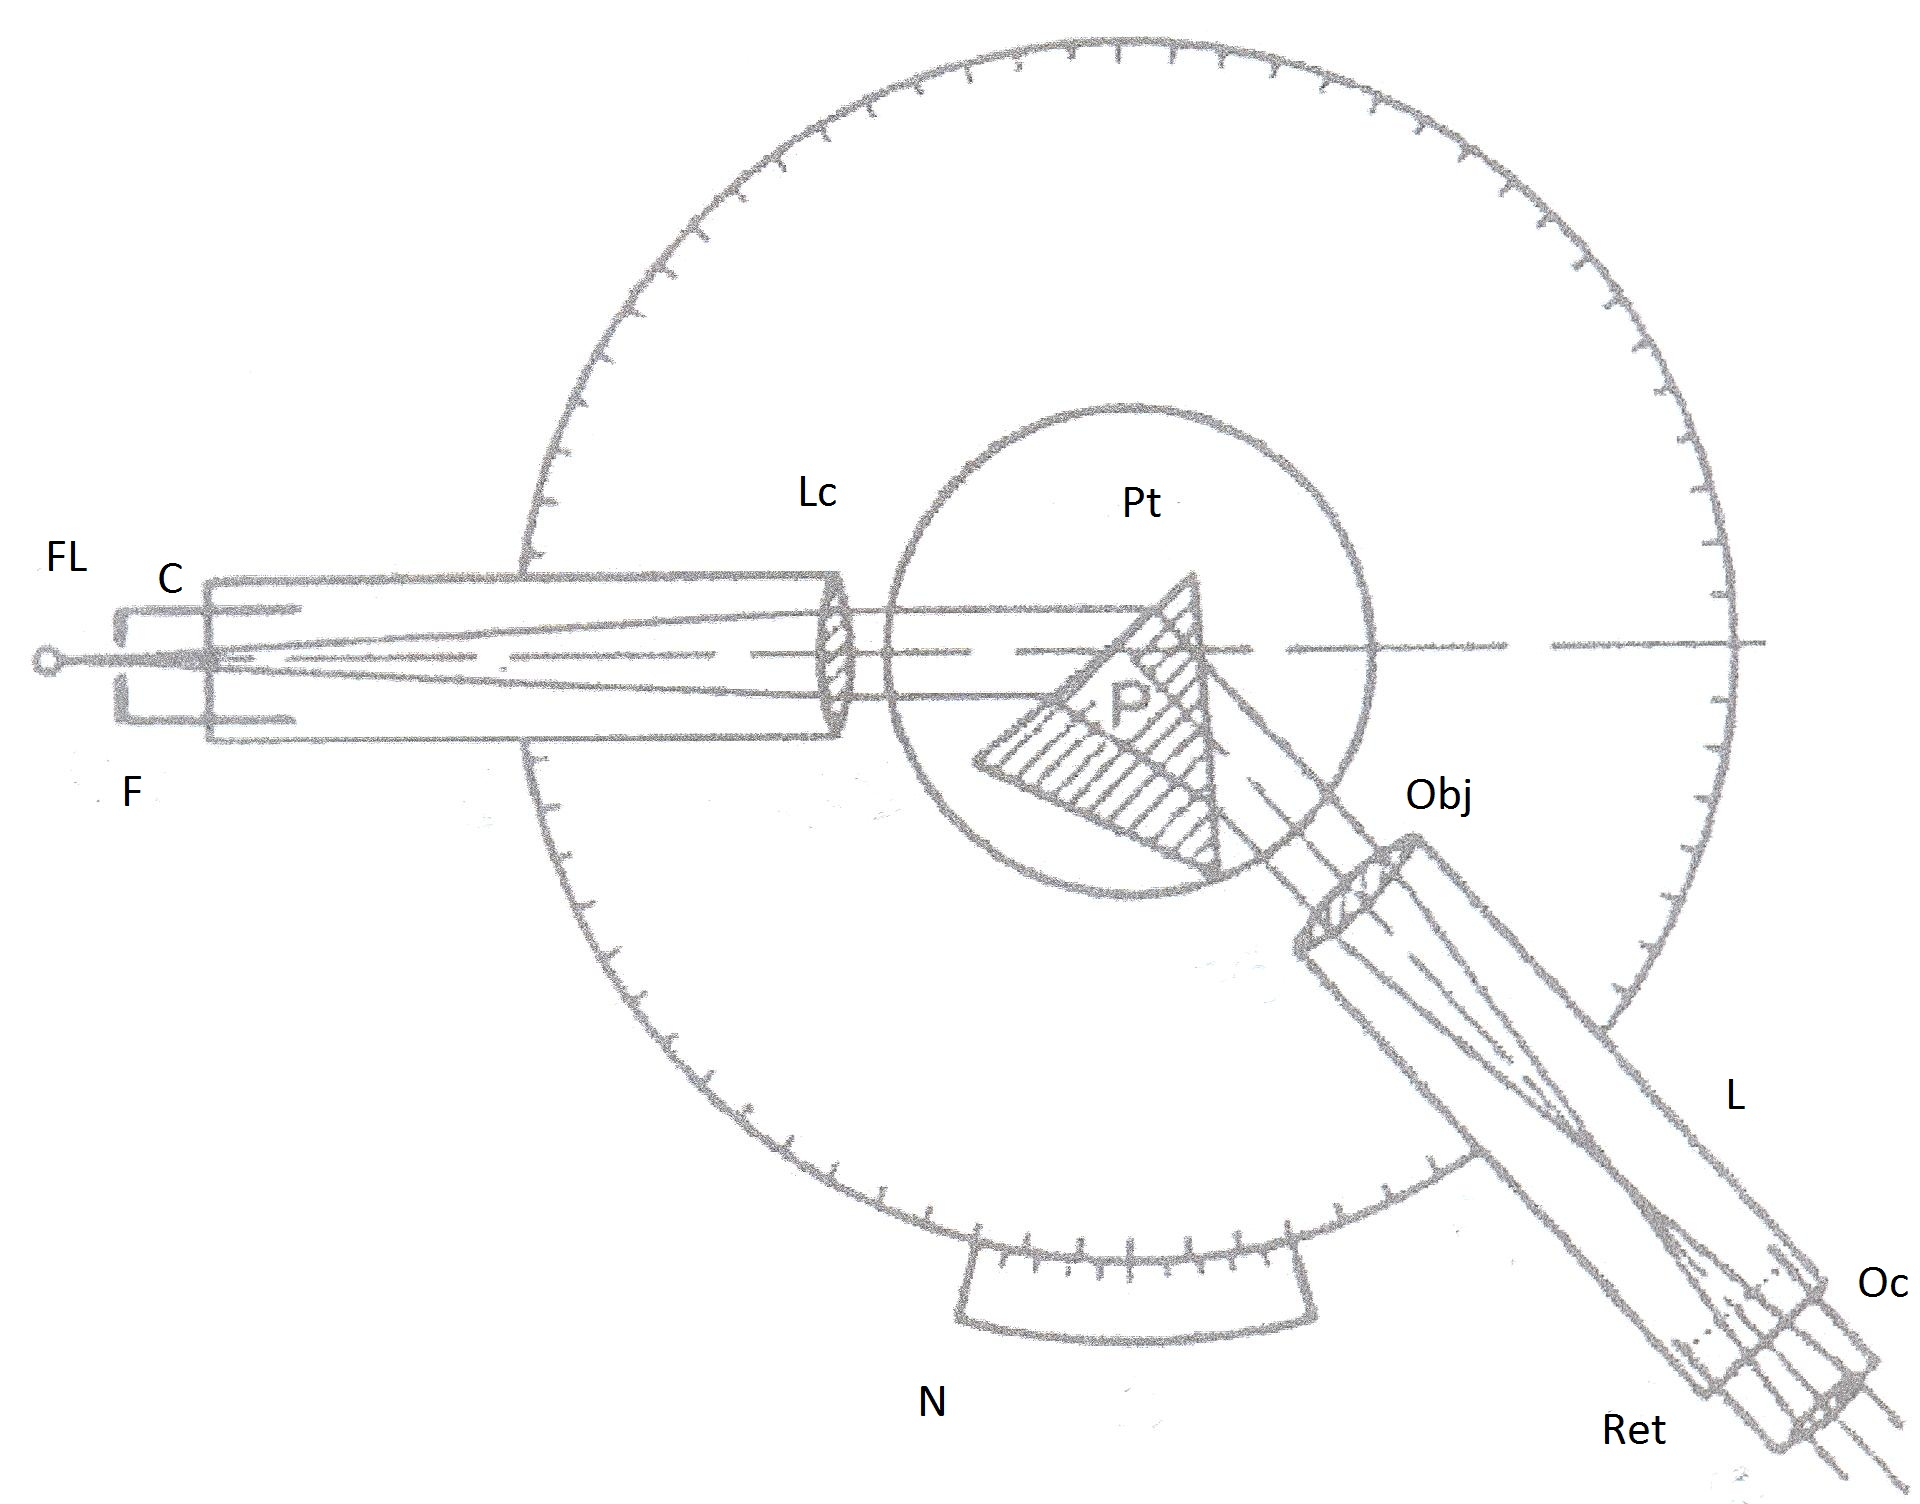
\includegraphics[width=0.55\textwidth]{babinet}
	\caption{Esquema do Goniómetro de Babinet. Legenda: FL-fonte luminosa, C-colimador, F-fenda, Lc-lente convergente do colimador, Pt-plataforma, P-Prisma, L-luneta, Obj-objetiva, Oc-ocular, Ret-retículo, N-nónio acoplado à luneta\label{fig:babinet}} 
\end{figure}

A luneta é constituída por dois elementos ópticos, uma lente convergente e uma ocular munida de retículo (dois fios cruzados perpendicularmente). A primeira lente produz no seu plano focal a imagem da fenda que é projetada no plano do retículo e ampliada pela ocular regulada pelo observador de modo a ver uma imagem focada da fenda. Quando se dispõe de um sistema de deteção (placa fotográfica ou um detetor, por exemplo uma célula fotoelétrica com um sistema de amplificação), este é colocado diretamente no plano focal da lente convergente e é retirada a ocular.
O prisma que se usa é em geral de seção reta triangular equilátera e, se nenhuma face está despolida, podem fazer-se leituras envolvendo cada um dos três ângulos. A aresta do ângulo definido pelas superfícies planas onde se produz a reflexão e transmissão deve ficar paralela à fenda(vertical).
A lâmpada espetral é uma fonte de luz policromática e discreta que contem dois elétrodos situados no interior de um invólucro (vidro em geral) onde existe uma substância “ativa”\footnote{Que dá o nome à lâmpada, e.g. Mercúrio, Hélio, Néon, etc.} em muito pequena quantidade numa atmosfera rarefeita. A alimentação que em geral é dedicada à lâmpada é de alta tensão e produz entre os elétrodos uma descarga que vaporiza, excita e ioniza a substância ativa. As diferentes excitações permitem transições radiativas que dão origem à emissão de um feixe constituido por diferentes comprimentos de onda bem definidos e que se encontram já muito bem identificados na Literatura. 
Todas as lâmpadas espetrais emitem no ultravioleta que é nocivo para a pele e olhos dos observadores, mas o vidro no interior do qual se dá a descarga absorve a maior parte destas radiações perigosas. Para reduzir os riscos, a lâmpada tem um invólucro em geral metálico apenas com uma abertura para permitir iluminar a fenda do goniómetro.

~
\newpage
\subsection{\sf Questões a responder ANTES da sessão de Laboratório:}
\begin{enumerate}
\item Obtenha uma imagem típica da dispersão da luz Branca num prisma triangular. O índice de refração, $n(\lambda)$, é uma função crescente ou decrescente?
\item Nessa figura de dispersão como faria para  identificar qual é a côr que está na posição de \emph{desvio mínimo}?
\item Se na montagem de laboratório substituir a lampada de descarga por uma de incandescência que imagem obteria com o goniometro?. 
\item O espectro de emissão do Hidrogéneo, na série de Balmer (transição $3 \to 2$) tem duas riscas no vermelho, respetivamente a $\lambda = 656.272\, nm$ e $\lambda = 656.2852\,nm$.
Qual a Resolução mínima de um instrumento (Espectrómetro) capaz de distinguir estas duas linhas?. Supondo que tem um prisma com aresta de $10\,cm$, calcule o 
o declive mínimo para $\left(\frac{\ud n}{\ud \lambda} \right)$?
\end{enumerate}


\section{\sf Protocolo Experimental}



\begin{enumerate}
\item Ligue  a  lâmpada  espetral  e  espere  10  a  15  minutos    até  que  se  estabeleça  o 
equilíbrio térmico no seu interior. 
\item Enquanto espera começe por regular a ocular da luneta do goniómetro. Para isso deve ver nitidamente com um 
olho  os fios do retículo e simultaneamente com o outro olho, ver um objeto no exterior da luneta afastado a cerca de 
$30\,cm$.  
\item Para  regular  a  objetiva,  observe  agora  um  objeto  no  “infinito” (no  laboratório 
escolha  um objeto  mais  afastado possível)  atuando  sobre  o  parafuso  da  luneta.  Regule  de  modo  a 
observar o objeto e o retículo bem focado e sem paralaxe. 
\item Coloque  a  luneta  alinhada de frente  do  colimador  e  regule  parafuso  do 
colimador de modo a observar a fenda focada quando iluminada pela lâmpada espetral. 
\item Verifique o nivelamento horizontal do goniómetro e da plataforma onde vai colocar o prisma com a ajuda de um nível de bolha. 
\item Observe a reflexão em cada face que define o ângulo do prisma e registe a posição angular 
correspondente a essas reflexões. Cada observador deve fazer três determinações usando o 
parafuso  micrométrico e centrando  a  imagem  da  fenda  com  o retículo  por  aproximação  à 
direita e à esquerda. 
\item  Observe  a  transmissão  do  feixe  através  do  prisma  com  o  feixe  incidente  numa  das  faces 
(envolvendo  o  ângulo  que  utilizou  no  ponto  anterior).  Deve  observar  agora  uma  série  de 
imagens da fenda, uma por cada côr, i.e comprimento de onda incidente.
\item Escolha uma dessas imagens e rodando o prisma obtenha um conjunto de valores que permita fazer um gráfico do ângulo de desvio, $\delta$, 
versus o ângulo de rotação do prisma (que por sua vez varia o ângulo de incidência, $i$). Verifique de existe de facto um mínimo.  
\item  Em seguida para cada côr, tem de rodar o prisma para que se obtenha a posição de desvio mínimo. Pode agora procurar finamente a posição de desvio mínimo 
com  o auxílio  do  parafuso  micrométrico  associado  à  plataforma  e  em  seguida,  com  o 
parafuso micrométrico associado à luneta, centrar a imagem no retículo. Faça pelo menos 
duas determinações de $\delta_{min}$ para cada cor. Repita este procedimento para a outra face do prisma. 
\item Conhecidos  os  valores  dos  comprimentos  de  onda  incidente, represente  graficamente  o 
índice de refração em função do comprimento de onda. Ajuste uma função polinomial à 
curva obtida. Através da 1ª derivada desta função, calcule o poder dispersivo do vidro para o comprimento de onda médio $\lambda$ das 
duas riscas amarelas do sódio ($\lambda \approx 589\,nm$). 
\item Faça uma estimativa da maior distância percorrida pelo feixe luminoso no prisma e calcule 
aproximadamente  o  poder  de  resolução  do  prisma  para  o  $\lambda$ referido  no  ponto  anterior. 
Compare este valor com o que obteria se usasse o mesmo feixe com uma rede de difração 
de 600 linhas por milímetro. 
\item Substitua no centro da plataforma do goniómetro o prisma por uma rede de difração de 
600 linhas por milímetro. Compare a separação angular $\Delta \theta$ das duas riscas mais próximas, 
observadas  com  a  rede  com  a  que  obteve  para  as  mesmas  riscas,  usando  o  prisma. 
Comente. 

\end{enumerate}

%\newpage
\section*{\sf Apêndice}
\subsection*{\sf Ângulo do Prisma}

Considere-se a incidência nas condições da Figura \ref{fig:angulo}.
A figura plana quadrangular $ABEC$ tem dois ângulos retos $ABE$ e $ECA$. Assim o ângulo $CAB$, $\alpha$, é suplementar do ângulo $BEC$ e portanto o ângulo externo em $E$ (assinalado na figura) tem o mesmo valor do ângulo do prisma.
Na figura plana quadrangular DBEC está definido um ângulo $θ$ que é o ângulo formado pelas direções dos raios refletidos na face $AB$ e $AC$. 
Entre os ângulos de incidência e $θ$ existe a relação 

 \begin{equation}
	\label{eq:soma}
	2\, \beta  + 2 \, \gamma + \theta = 2 \, \pi
\end{equation}

e entre os ângulos de $DBEC$ 
 \begin{equation}
	\label{eq:soma2}
	\beta  +  \gamma + \theta  + \pi - \alpha= 2 \, \pi
\end{equation}

O sistema destas duas equações permite obter 
 \begin{equation}
	\label{eq:alpha}
	\alpha=  \theta /2 
\end{equation}

\subsection*{\sf Desvio mínimo}
Supondo um prisma que tem um índice de refração que em relação ao meio em que está imerso $n$, na configuração da Figura \ref{fig:desvio}, os feixes que são transmitidos através do mesmo sofrem um desvio $\delta(\lambda)$. Os ângulos  $\alpha$ e de desvio $\delta $  são exteriores respetivamente aos triângulos $BCD$ (em $D$) e $BEC$ (em $E$) e portanto 


\begin{IEEEeqnarray}{rCl}
\delta &  =  &  (i_1 - t_1) +  (t_2 - i_2) \\
\alpha &  =  &  t_1  + i_2 \label{eq:soma3}
\end{IEEEeqnarray}

o que permite obter 
 \begin{equation}
	\label{eq:delta}
	\delta   =    i_1  +  t_2  - \alpha 
\end{equation}

Estes ângulos satisfazem à lei de Snell-Descartes da transmissão

 \begin{equation}
	\label{eq:snell}
	n = \frac{\sin i_1}{\sin t_1}  =  \frac{\sin t_2}{\sin i_2}  
\end{equation}

No caso geral o ângulo $\delta$ depende do ângulo de incidência $i_1$ e pode provar-se que a função envolvida tem uma estacionariedade. Para encontrar o \emph{desvio mínimo} $\delta_{min}$, calculemos pois a derivada de $\delta$ em relação a $i_1$ (expressão \ref{eq:delta}).

 \begin{equation}
	\label{eq:deriv}
	\frac{\ud \delta}{\ud i_1}   =  1 + 	\frac{\ud t_2}{\ud i_1} 
\end{equation}

Obtendo $\sin i_1$ e $\sin t_2$ da relação (\ref{eq:snell}) e aplicando-lhe derivada em ordem a $i_1$ é-se conduzido a 
\begin{IEEEeqnarray}{rCl}
\cos i_1 &  =  & n \,\cos t_1 \cdot  \frac{\ud t_1}{\ud i_1} 	\label{eq:deriv2} \\
\cos t_2  \cdot   \frac{\ud t_2}{\ud i_1}  &  =  & n \, \cos i_2  \cdot  \frac{\ud i_2}{\ud i_1} 	\label{eq:deriv3}
\end{IEEEeqnarray}

Mas atendendo à relação (\ref{eq:soma3})
 \begin{equation}
	\label{eq:deriv4}
	\frac{\ud t_1}{\ud i_1}  = - \frac{\ud i_2}{\ud i_1} 
\end{equation}

e combinando (\ref{eq:deriv2}), (\ref{eq:deriv3}) e (\ref{eq:deriv4}) obtém-se
 \begin{equation}
	\label{eq:deriv5}
	\frac{\ud t_2}{\ud i_1}  = - \frac{\cos i_2\,\cos i_1}{\cos t_2\,\cos t_1} 
\end{equation}

e a relação (\ref{eq:deriv}) vem

\begin{equation}
	\label{eq:deriv6}
	\frac{\ud \delta}{\ud i_1}   = 1-  \frac{\cos i_2\,\cos i_1}{\cos t_2\,\cos t_1} 
\end{equation}
Esta função admite um zero para
\begin{equation}
	\label{eq:deriv_0}
	{\cos i_2\,\cos i_1}={\cos t_2\,\cos t_1} 
\end{equation}

Atendendo a (\ref{eq:snell}) e à relação entre coseno e seno obtém-se
\begin{equation}
	\label{eq:deriv_1}
	\sin^2 t_1 \cdot  (1 - n^2)  = \sin^2 i_2 \cdot  (1 - n^2)
\end{equation}

que para os ângulos considerados ($\le  \pi/2)$ e para $n\ne 1$ implica que 

\begin{IEEEeqnarray}{rCl}
t_1  &  =  & i_2 = t\\
i_1  &  =  & t_2 = i
\end{IEEEeqnarray}


Assim para $\frac{\ud \delta}{\ud i} =0 $  (que provaremos ser um mínimo)
\begin{equation}
	\label{eq:deltvmin}
	\delta_{min} = 2\,i- 2\,t = 2\,i - \alpha
\end{equation}

o que permite calcular $t$ a partir do ângulo do prisma ($t = \alpha / 2$) e $i$ a partir do ângulo de desvio mínimo e do ângulo do prisma ($i = (\alpha + \delta_{min} ) / 2$) e consequentemente obter a relação (\ref{eq:desviomim}) para o cálculo do índice de refração.

É necessário calcular  $\frac{\ud^2 \delta}{\ud i^2} =0 $ e verificar se é uma quantidade positiva ou negativa para os valores que anulam a primeira derivada com o objetivo de saber se a estacionariedade é um mínimo,  máximo  ou um ponto de inflexão.
Aplicando derivada em ordem a $i$ à expressão (\ref{eq:deriv6}) obtém-se

\begin{equation}
	\label{eq:d2eriv}
	\frac{\ud^2 \delta}{\ud i_1^2}   =   	\frac{\ud }{\ud i_1} \left(-  \frac{\cos i_2\,\cos i_1}{\cos t_2\,\cos t_1} \right)
\end{equation}

em que todos os argumentos das funções coseno dependem de $i_1$.
obtém-se 4 parcelas que são: 

\begin{IEEEeqnarray}{rCl}
 \frac{\cos i_1}{\cos t_2\,\cos t_1} \frac{\ud }{\ud i_1} \cos i_2 &  =  & 
 \frac{\cos i_1}{\cos t_2\,\cos t_1} (-\sin i_2) \frac{\ud i_2}{\ud i_1} 	\label{eq:d2eriv_a}\\
%
 \frac{\cos i_2}{\cos t_2\,\cos t_1} \frac{\ud }{\ud i_1} \cos i_1 &  =  & 
 \frac{\cos i_2}{\cos t_2\,\cos t_1} (-\sin i_1)  \label{eq:d2eriv_b} \\
 \frac{\cos i_2\,\cos i_1}{\cos t_1}  \frac{\ud }{\ud i_1} (\cos t_2)^{-1} &  =  & 
  \frac{\cos i_2\,\cos i_1}{\cos t_1} \sin t_2 (\cos t_2)^{-2} \frac{\ud t_2}{\ud i_1}\label{eq:d2eriv_c}\\
  \frac{\cos i_2\,\cos i_1}{\cos t_2}  \frac{\ud }{\ud i_1} (\cos t_1)^{-1}  &  =  & 
  \frac{\cos i_2\,\cos i_1}{\cos t_2} \sin t_1 (\cos t_1)^{-2} \frac{\ud t_1}{\ud i_1} \label{eq:d2eriv_d}
\end{IEEEeqnarray}

Atendendo a (\ref{eq:deriv2}) e (\ref{eq:deriv4}) substituidos em (\ref{eq:d2eriv_a}) e em (\ref{eq:d2eriv_c}) e a (\ref{eq:deriv5}) substituido em (\ref{eq:d2eriv_d}), as 4 parcelas conduzem respetivamente às expressões seguintes que são simplificadas quando se substitui $n$ (\ref{eq:snell}) e se impõem as condições que foram obtidas para o zero de   $\frac{\ud \delta}{\ud i_1} $ 

\begin{IEEEeqnarray}{rCl}
 \frac{\cos i_1}{\cos t_2\,\cos t_1} (-\sin i_2) \frac{\cos i_1}{n\, \cos t_1}  &  =  & 	
    \frac{\sin^2 t}{\cos^2 t}  \frac{\cos i}{\sin i} \\
%
 \cdots &  =  & -\frac{\sin i}{\cos i} \\
 \cdots &  =  & -\frac{\sin i}{\cos i} \\
 \cdots &  =  & 	  \frac{\sin^2 t}{\cos^2 t}  \frac{\cos i}{\sin i} 
\end{IEEEeqnarray}

Assim obtém-se 

\begin{equation}
	\label{eq:d22e}
	\frac{\ud^2 \delta}{\ud i_1^2}   =   -2 \tan^2 t  \, \frac{1}{\tan i} + 2\tan i = 2 \, \tan i 
	\left(1 - \frac{\tan^2 t}{\tan^2 i} \right)
\end{equation}
Esta expressão é positiva para $ \tan^2 t < \tan^2 i $ o que implica $t < i$ ($i, t \le \pi/2$), ie, para $n > 1$ e é negativa para $n < 1$. No caso do prisma de vidro imerso no ar $n > 1$ e portanto (\ref{eq:d22e}) será positiva o que confirma que a condição de estacionariedade corresponde a um mínimo.

\subsection*{\sf Poder de resolução do prisma}

A capacidade de observar separadamente dois comprimentos de onda muito próximos está relacionada com a variação do ângulo de desvio $\delta$ com o comprimento de onda λ que se designa por dispersão angular   
$\frac{\ud \delta}{\ud \lambda}$ e que depende do coeficiente de dispersão  $\frac{\ud n}{\ud \lambda}$ na forma  

\begin{equation}
	\label{eq:poder_res}
	\frac{\ud \delta}{\ud \lambda} =\frac{\ud \delta}{\ud n} \, \frac{\ud n}{\ud \lambda}
\end{equation}

Atendendo a (\ref{eq:delta}) $\frac{\ud \delta}{\ud n} = \frac{\ud t_2}{\ud n}$ (para $\alpha$ e $i_1$ constantes). Derivando a relação (\ref{eq:snell}) em ordem a $n$ obtém-se

\begin{IEEEeqnarray}{rCl}
\cos t_2 =  \frac{\ud t_2}{\ud n}  &  =  &  \sin t_2 + n\, \cos i_2  \frac{\ud i_2}{\ud n}\\
0 &  =  &  \sin t_1 +  n\, \cos t_1  \frac{\ud t_1}{\ud n}
\end{IEEEeqnarray}

Obtém-se assim 

\begin{IEEEeqnarray}{rCl}
\frac{\ud \delta}{\ud n}    &  =  &   \frac{\sin i_2}{\cos t_2} +  \frac{\sin t_1\; \cos i_2}{\cos t_2 \; \cos t_1 } =  \frac{\sin \alpha}{\cos t_2 \; \cos t_1 } \\
\frac{\ud \delta}{\ud \lambda}    &  =  & \frac{\ud n}{\ud \lambda} \frac{\sin \alpha}{\cos t_2 \; \cos t_1 } 
\end{IEEEeqnarray}

Considerando um feixe paralelo de largura $l_1$ como se indica na Figura \ref{fig:feixe}, que incide no prisma segundo um ângulo $i_1$ e que emerge segundo $t_2$ com largura $l_2$, fazendo um percurso máximo no prisma $l$, pode provar-se (os senos dos ângulos de um triângulo são diretamente proporcionais aos lados opostos) que 


\begin{figure}[!htb]  \centering 
	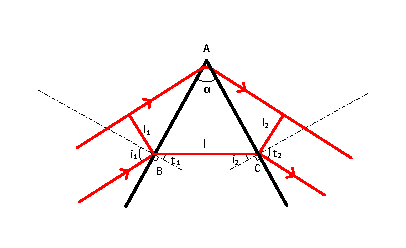
\includegraphics[width=0.6\textwidth]{feixe}
	\caption{Trajeto de um feixe luminoso paralelo num prisma. \label{fig:feixe}} 
\end{figure}

\begin{equation}
	\label{eq:sin_alpha}
	\frac{\sin \alpha}{l}= \frac{\sin (\pi/2 - t_1)} {AC}
\end{equation}

e atendendo a que $l_2= AC \cos t_2$  obtém-se que 

\begin{equation}
	\label{eq:delt_lamd}
	\frac{\ud \delta}{\ud \lambda}  =  \frac{\ud n}{\ud \lambda} \frac{l}{l_2}
\end{equation}

Assim uma pequena variação de comprimento de onda $\Delta \lambda$ produz uma variação do ângulo de desvio $\Delta \delta$  tal que 

\begin{equation}
	\label{eq:Delt_delta}
	\Delta \delta =  \frac{\ud n}{\ud \lambda} \frac{l}{l_2} \Delta \lambda 
\end{equation}

O critério de Rayleigh para que dois comprimentos de onda estejam resolvidos, ie possam ser detetados separadamente, é que o máximo de intensidade de um deles coincida com o mínimo de intensidade do outro (Figura \ref{fig:gauss})

\begin{figure}[ht]  \centering 
	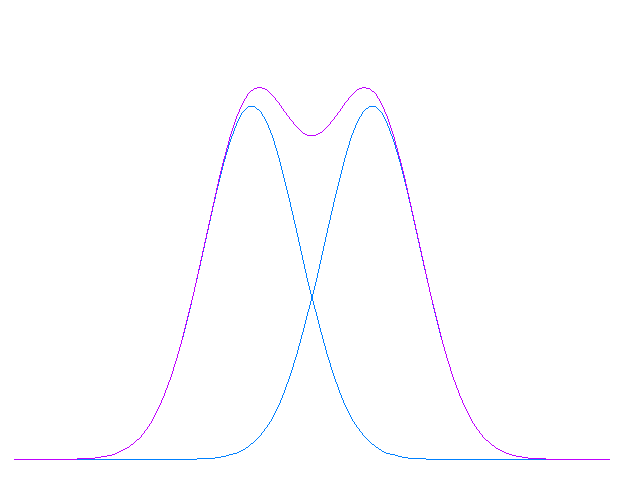
\includegraphics[width=0.6\textwidth]{gauss}
	\caption{Critério de Rayleigh da resolução de duas riscas espetrais (a vermelho a soma da intensidade das riscas. \label{fig:gauss}} 
\end{figure}

Ver-se-á no trabalho de Difração que o primeiro mínimo de intensidade da figura de difração de uma fenda de largura $l_2$ dista angularmente do máximo principal de  $\sin \theta = \lambda/l_2$.
Para dois comprimentos de onda muito próximos $\sin  \theta \approx \theta $ que neste caso é o desvio angular $\Delta \delta$. Assim $\Delta \delta= \lambda / l_2$ e obtém-se para a resolução do prisma: 

~\begin{equation}
	\label{eq:resolup}
	R_\lambda  =  \frac{\lambda}{\Delta \lambda} = l \left(\frac{\ud n}{\ud \lambda} \right )_\lambda 
\end{equation}



\end{document} 